To numerically solve a set of PDEs, iterative methods (finite difference, finite volume or finite element methods) are frequently used to approximate the solution through a discretized (step by step) phenomena. Thus, the continuous time and space domains are discretized so that a set of numerical computations are iteratively (time discretization) applied onto a mesh (space discretization). In other words, the PDEs are transformed to a set of numerical computations applied at each time step on all elements of the discretized space domain. Among those numerical computations is found a set of numerical schemes, also called \textit{stencil computations}, and a set of auxiliary computations also needed to perform the simulation, and also called \emph{local computations}.
This section gives formal definitions of a \textit{stencil program} and its computations. Then, the different parallelization techniques which can be applied on such program, are presented.

%-------------------------------------
\subsection{Time, mesh and data}

$\Omega=\mathbb{R}^n$ is the continuous space domain of a numerical simulation. Any geo-referenced point in this space can be represented.

A mesh $\mathcal{M}$ defines the discretization of the continuous space domain $\Omega$ of a set of PDEs and is defined as follows.

\begin{mydef}
\textit{A mesh is a connected undirected graph $\mathcal{M}=(V,E)$, where $V\subset \Omega$ is the set of vertices and $E\subseteq V^2$ the set of edges. The set of edges $E$ of a mesh $\mathcal{M}=(V,E)$ does not contain bridges.}
\end{mydef}
\begin{figure}[!h]\begin{center}
  \resizebox{8cm}{!}{\includegraphics{./images/maillages.pdf}}
  \caption{From left to right, Cartesian, curvilinear and unstructured meshes.}
  \label{fig:mesh}
\end{center}\end{figure}
A mesh can be structured (as Cartesian or curvilinear meshes), unstructured, regular or irregular (without the same topology for each element) and hybrid as illustrated in Figure~\ref{fig:mesh}.

\noindent \textbf{Definitions}
%\begin{mydef}
\begin{itemize}
\item An entity $e$ of a mesh $\mathcal{M}=(V,E)$ is a subset of its vertices and edges, $e\subset (V\cup E)$. 
\item The set of mesh entities, of a same given type, is denoted $E$ such that $E\subset \mathcal{P}(V\cup E)$. 
\item Finally the set of mesh entities of a simulation is denoted $\mathcal{E}$.
\end{itemize}
%\end{mydef}

For example, in a 2D Cartesian mesh a first kind of entities are the cells, they can be defined as all sets containing exactly four vertices and four edges connected as a cycle. Another kind of entities simply are the vertices ($V$) and can be defined as all singletons formed of a single vertex of $V$.

\medskip
This covers the space discretization, however another dimension manipulated in simulations that has to be discretized is the time dimension.

\noindent \textbf{Definitions}
%\begin{mydef}
\begin{itemize}
\item $\mathcal{T}=\mathbb{R}$ is the continuous time domain of a numerical simulation.
\item The discretization of the continuous time domain $\mathcal{T}$ is denoted $T$ such that $\forall\mbox{ }t_i\mbox{, }t_{i+1} \in T\mbox{, }\exists\mbox{ }\Delta t \in \mathbb{R}$\mbox{, }$t_{i+1} = t_i + \Delta t$.
\end{itemize}
%\end{mydef}

$T$ is responsible for the iteration time steps of the numerical simulation. A numerical simulation though does not run forever and must be stopped at some point. Some simulations choose a fix number of time iteration, others compute a \emph{convergence} criteria at the end of each time iteration to determine if the simulation has to continue. A convergence criteria is computed by a reduction computation that will be detailed in the next section.

In a numerical simulation a set of data elements, or quantities, are applied onto the mesh and represent the set of values to compute, or to use, for computation.

\noindent \textbf{Definitions}
%\begin{mydef}
\begin{itemize}
\item A quantity is a function $\delta: E_{\delta} \mapsto V_{\delta}$ which associates each entity of a type $e\in E_{\delta}$ to a value $v\in V_{\delta}$ where $V_{\delta}$ is the data type, typically $\mathbb{R}$ or $\mathbb{C}$.
\item The set of quantities applied onto the mesh is denoted $\Delta$.
\item In the rest of this paper, the type of mesh entities on which a quantity $\delta$ is mapped is denoted $entity(\delta)=E_{\delta}$.
\end{itemize}
%\end{mydef}

Another approach closer to that taken in applied mathematics would have been to define $\delta$ functions over $E_{\delta} \times T$; however the approach chosen in this paper where a distinct function is defined for each time-step better matches the implementation of numerical simulations where the outer loop iterates over time and where only a few time-steps of quantity values are stored.

%-----------------------
\subsection{Computations}

In this section are considered two different types of computations, a reduction or a numerical kernel. 

\noindent \textbf{Definitions}
%\begin{mydef}
\begin{itemize}
\item A computation domain $D$ is a subpart of mesh entities of a given type, $D \subset E \in \mathcal{E}$.
\item The set of computation domains of a numerical simulation is denoted $\mathcal{D}$.
\item A neighborhood $n$ is a function which for a given entity $e \in E_i$, returns a set of $m$ entities in $E_j$, $n : E_i \rightarrow E_j^m$. It is possible that $E_i = E_j$.
\item The set of neihborhood functions in a numerical simulation is denoted $\mathcal{N}$.
\item A set of data to read and used in a computation is denoted $R \subset \Delta \times \mathcal{N}$. It is the set of pairs $(r,n)$, where $r \in \Delta$ and $n$ is a neighborhood function such that $n : E_i \rightarrow entity(r)^m$.
\item A numerical expression $\text{exp}_{w}: entity(w) \times R \rightarrow V_{w}$ is a function that computes the value of the written quantity $w \in \Delta$ for a given entity $e \in entity(w)=E$, using a set of input data $R$.
\item A computation kernel $k$ of a numerical simulation is defined as $k(R,w,\text{exp},D)$, where $R \subset \Delta \times \mathcal{N}$ is the set of data read, $w \in \Delta$ is the unique data written, $\text{exp}$ is a numerical expression, and $D \in \mathcal{D}$.
\end{itemize}
%\end{mydef}
%If the number of computations in $\Gamma$ is $card(\Gamma)=n$, such that $\bigcup_{i=0}^{n-1}c_i = \Gamma$, then $\bigcup_{i=0}^{m-1}R_i \cup w_i \subseteq \Delta$.

Most of the time we can dissociate two types of kernel computations.

\noindent \textbf{Definitions}
%\begin{mydef}
\begin{itemize}
\item We denote by $identity$ the identity function $x=x$.
\item A kernel computation $k(R,w,\text{exp},D) \in \Gamma$ is a stencil kernel $\iff \exists (r,n) \in R$ such that $n \neq identity$.
\item A kernel computation $k(R,w,\text{exp},D) \in \Gamma$ is a local kernel $\iff \forall (r,n) \in R$, $n = identity$.
\item The set of $n$ ordered computations of a numerical simulation is denoted $\Gamma = [k_i]_{0 \leq i \leq n-1}$, such that $\forall k_i,k_j \in \Gamma$, if $i \leq j$, then $k_i$ is computed before $k_j$.
\end{itemize}

A reduction computation is typically used to compute the convergence criteria of the time loop of the simulation. Occasionally reductions can also be performed during a time iteration. This last usage is typically done to place a conditionnal branch to chose one computation or another. This paper only study the use of reduction computations as convergence citerion.

\noindent \textbf{Definitions}
%\begin{mydef}
\begin{itemize}
\item A reduction computation is defined as the triplet $red(R,)$
\item ...
\item A \textit{multi-stencil program} is defined by the sextuplet $\mathcal{MSP}(T,\mathcal{M},\mathcal{E},\mathcal{D},\Delta,\Gamma)$.
\end{itemize}
%\end{mydef}


For example, in Figure~\ref{fig:ex1}, assuming the computation domain (full lines) is denoted $dc1$ and the stencil shape is $n1$, the stencil kernel can be defined as:
\begin{equation*}
R: \{(B,n1)\}, \quad w: A, \quad d: dc1,
\end{equation*}
\begin{equation*}
exp: A(x,y)=B(x+1,y)+B(x-1,y)+B(x,y+1)+B(x,y-1).
\end{equation*}
On the other hand, in the example of Figure~\ref{fig:ex2}, assuming the computation domain is $dc2$ and the stencil shape is $n2$, the stencil kernel is defined as:
\begin{equation*}
R: \{(C,n2),(A,identity)\}, \quad w: A, \quad d: dc2,
\end{equation*}
\begin{equation*}
exp: A(x,y)=A(x,y)+C(x1,y1)+C(x1+1,y1).
\end{equation*}

\begin{figure}
\begin{center}
\subfloat[Mesh and mesh domains.\label{fig:mesh}]{
\resizebox{8cm}{!}{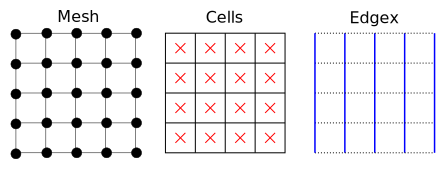
\includegraphics{./images/mesh.pdf}}
}\\
\hspace{10pt}
\subfloat[4-neighborhood stencil.\label{fig:ex1}]{
\resizebox{5cm}{!}{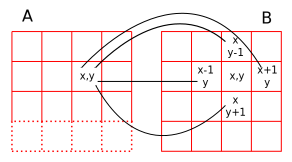
\includegraphics{./images/stencil1.pdf}}
}
\vspace{20pt}
\subfloat[4-neighborhood stencil.\label{fig:ex2}]{
\resizebox{5cm}{!}{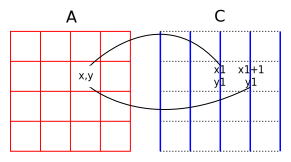
\includegraphics{./images/stencil2.pdf}}
}
\end{center}
\caption{(a) a Cartesian mesh and two kind of mesh entities, (b) an example of stencil kernel on cells, (c) an example of stencil kernel on two different entities of the mesh.}
\label{fig:gspmsp}
\end{figure}

A stencil program and stencil and local computations have been formally defined in this section. This formalism is used in the next Section to define two parallelization techniques of a multi-stencil program.


